\ifx\allfiles\undefined
\documentclass[12pt, a4paper, oneside, UTF8]{ctexbook}
\def\path{../../config}
\usepackage{amsmath}
\usepackage{amsthm}
\usepackage{amssymb}
\usepackage{array}
\usepackage{xcolor}
\usepackage{graphicx}
\usepackage{mathrsfs}
\usepackage{enumitem}
\usepackage{geometry}
\usepackage[colorlinks, linkcolor=black]{hyperref}
\usepackage{stackengine}
\usepackage{yhmath}
\usepackage{extarrows}
\usepackage{tikz}
\usepackage{pgfplots}
\usepackage{asymptote}
\usepackage{float}
\usepackage{fontspec} % 使用字体

\setmainfont{Times New Roman}
\setCJKmainfont{LXGWWenKai-Light}[
    SlantedFont=*
]

\everymath{\displaystyle}

\usepgfplotslibrary{polar}
\usepackage{subcaption}
\usetikzlibrary{decorations.pathreplacing, positioning}

\usepgfplotslibrary{fillbetween}
\pgfplotsset{compat=1.18}
% \usepackage{unicode-math}
\usepackage{esint}
\usepackage[most]{tcolorbox}

\usepackage{fancyhdr}
\usepackage[dvipsnames, svgnames]{xcolor}
\usepackage{listings}

\definecolor{mygreen}{rgb}{0,0.6,0}
\definecolor{mygray}{rgb}{0.5,0.5,0.5}
\definecolor{mymauve}{rgb}{0.58,0,0.82}
\definecolor{NavyBlue}{RGB}{0,0,128}
\definecolor{Rhodamine}{RGB}{255,0,255}
\definecolor{PineGreen}{RGB}{0,128,0}

\graphicspath{ {figures/},{../figures/}, {config/}, {../config/} }

\linespread{1.6}

\geometry{
    top=25.4mm, 
    bottom=25.4mm, 
    left=20mm, 
    right=20mm, 
    headheight=2.17cm, 
    headsep=4mm, 
    footskip=12mm
}

\setenumerate[1]{itemsep=5pt,partopsep=0pt,parsep=\parskip,topsep=5pt}
\setitemize[1]{itemsep=5pt,partopsep=0pt,parsep=\parskip,topsep=5pt}
\setdescription{itemsep=5pt,partopsep=0pt,parsep=\parskip,topsep=5pt}

\lstset{
    language=Mathematica,
    basicstyle=\tt,
    breaklines=true,
    keywordstyle=\bfseries\color{NavyBlue}, 
    emphstyle=\bfseries\color{Rhodamine},
    commentstyle=\itshape\color{black!50!white}, 
    stringstyle=\bfseries\color{PineGreen!90!black},
    columns=flexible,
    numbers=left,
    numberstyle=\footnotesize,
    frame=tb,
    breakatwhitespace=false,
} 

\lstset{
    language=TeX, % 设置语言为 TeX
    basicstyle=\ttfamily, % 使用等宽字体
    breaklines=true, % 自动换行
    keywordstyle=\bfseries\color{NavyBlue}, % 关键字样式
    emphstyle=\bfseries\color{Rhodamine}, % 强调样式
    commentstyle=\itshape\color{black!50!white}, % 注释样式
    stringstyle=\bfseries\color{PineGreen!90!black}, % 字符串样式
    columns=flexible, % 列的灵活性
    numbers=left, % 行号在左侧
    numberstyle=\footnotesize, % 行号字体大小
    frame=tb, % 顶部和底部边框
    breakatwhitespace=false % 不在空白处断行
}

% \begin{lstlisting}[language=TeX] ... \end{lstlisting}

% 定理环境设置
\usepackage[strict]{changepage} 
\usepackage{framed}

\definecolor{greenshade}{rgb}{0.90,1,0.92}
\definecolor{redshade}{rgb}{1.00,0.88,0.88}
\definecolor{brownshade}{rgb}{0.99,0.95,0.9}
\definecolor{lilacshade}{rgb}{0.95,0.93,0.98}
\definecolor{orangeshade}{rgb}{1.00,0.88,0.82}
\definecolor{lightblueshade}{rgb}{0.8,0.92,1}
\definecolor{purple}{rgb}{0.81,0.85,1}

\theoremstyle{definition}
\newtheorem{myDefn}{\indent Definition}[section]
\newtheorem{myLemma}{\indent Lemma}[section]
\newtheorem{myThm}[myLemma]{\indent Theorem}
\newtheorem{myCorollary}[myLemma]{\indent Corollary}
\newtheorem{myCriterion}[myLemma]{\indent Criterion}
\newtheorem*{myRemark}{\indent Remark}
\newtheorem{myProposition}{\indent Proposition}[section]

\newenvironment{formal}[2][]{%
	\def\FrameCommand{%
		\hspace{1pt}%
		{\color{#1}\vrule width 2pt}%
		{\color{#2}\vrule width 4pt}%
		\colorbox{#2}%
	}%
	\MakeFramed{\advance\hsize-\width\FrameRestore}%
	\noindent\hspace{-4.55pt}%
	\begin{adjustwidth}{}{7pt}\vspace{2pt}\vspace{2pt}}{%
		\vspace{2pt}\end{adjustwidth}\endMakeFramed%
}

\newenvironment{definition}{\vspace{-\baselineskip * 2 / 3}%
	\begin{formal}[Green]{greenshade}\vspace{-\baselineskip * 4 / 5}\begin{myDefn}}
	{\end{myDefn}\end{formal}\vspace{-\baselineskip * 2 / 3}}

\newenvironment{theorem}{\vspace{-\baselineskip * 2 / 3}%
	\begin{formal}[LightSkyBlue]{lightblueshade}\vspace{-\baselineskip * 4 / 5}\begin{myThm}}%
	{\end{myThm}\end{formal}\vspace{-\baselineskip * 2 / 3}}

\newenvironment{lemma}{\vspace{-\baselineskip * 2 / 3}%
	\begin{formal}[Plum]{lilacshade}\vspace{-\baselineskip * 4 / 5}\begin{myLemma}}%
	{\end{myLemma}\end{formal}\vspace{-\baselineskip * 2 / 3}}

\newenvironment{corollary}{\vspace{-\baselineskip * 2 / 3}%
	\begin{formal}[BurlyWood]{brownshade}\vspace{-\baselineskip * 4 / 5}\begin{myCorollary}}%
	{\end{myCorollary}\end{formal}\vspace{-\baselineskip * 2 / 3}}

\newenvironment{criterion}{\vspace{-\baselineskip * 2 / 3}%
	\begin{formal}[DarkOrange]{orangeshade}\vspace{-\baselineskip * 4 / 5}\begin{myCriterion}}%
	{\end{myCriterion}\end{formal}\vspace{-\baselineskip * 2 / 3}}
	

\newenvironment{remark}{\vspace{-\baselineskip * 2 / 3}%
	\begin{formal}[LightCoral]{redshade}\vspace{-\baselineskip * 4 / 5}\begin{myRemark}}%
	{\end{myRemark}\end{formal}\vspace{-\baselineskip * 2 / 3}}

\newenvironment{proposition}{\vspace{-\baselineskip * 2 / 3}%
	\begin{formal}[RoyalPurple]{purple}\vspace{-\baselineskip * 4 / 5}\begin{myProposition}}%
	{\end{myProposition}\end{formal}\vspace{-\baselineskip * 2 / 3}}


\newtheorem{example}{\indent \color{SeaGreen}{Example}}[section]
\renewcommand{\proofname}{\indent\textbf{\textcolor{TealBlue}{Proof}}}
\NewEnviron{solution}{%
	\begin{proof}[\indent\textbf{\textcolor{TealBlue}{Solution}}]%
		\color{blue}% 设置内容为蓝色
		\BODY% 插入环境内容
		\color{black}% 恢复默认颜色(可选,避免影响后续文字)
	\end{proof}%
}

% 自定义命令的文件

\def\d{\mathrm{d}}
\def\R{\mathbb{R}}
%\newcommand{\bs}[1]{\boldsymbol{#1}}
%\newcommand{\ora}[1]{\overrightarrow{#1}}
\newcommand{\myspace}[1]{\par\vspace{#1\baselineskip}}
\newcommand{\xrowht}[2][0]{\addstackgap[.5\dimexpr#2\relax]{\vphantom{#1}}}
\newenvironment{mycases}[1][1]{\linespread{#1} \selectfont \begin{cases}}{\end{cases}}
\newenvironment{myvmatrix}[1][1]{\linespread{#1} \selectfont \begin{vmatrix}}{\end{vmatrix}}
\newcommand{\tabincell}[2]{\begin{tabular}{@{}#1@{}}#2\end{tabular}}
\newcommand{\pll}{\kern 0.56em/\kern -0.8em /\kern 0.56em}
\newcommand{\dive}[1][F]{\mathrm{div}\;\boldsymbol{#1}}
\newcommand{\rotn}[1][A]{\mathrm{rot}\;\boldsymbol{#1}}

\newif\ifshowanswers
\showanswerstrue % 注释掉这行就不显示答案

% 定义答案环境
\newcommand{\answer}[1]{%
    \ifshowanswers
        #1%
    \fi
}

% 修改参数改变封面样式,0 默认原始封面、内置其他1、2、3种封面样式
\def\myIndex{0}


\ifnum\myIndex>0
    \input{\path/cover_package_\myIndex} 
\fi

\def\myTitle{考研数学笔记}
\def\myAuthor{Weary Bird}
\def\myDateCover{\today}
\def\myDateForeword{\today}
\def\myForeword{相见欢·林花谢了春红}
\def\myForewordText{
    林花谢了春红,太匆匆。
    无奈朝来寒雨晚来风。
    胭脂泪,相留醉,几时重。
    自是人生长恨水长东。
}
\def\mySubheading{以姜晓千强化课讲义为底本}


\begin{document}
\else
\fi

\chapter{二重积分}
\section{二重积分的概念}

\begin{remark}
    二重积分的定义
    $$
    \lim_{n\to\infty}\sum_{i=1}^{n}\sum_{j=1}^{n}f(\frac{i}{n},\frac{j}{n})\cdot\frac{1}{n}\frac{1}{n}=\int_{0}^{1}\int_{0}^{1}f(x,y)\d x\d y
    $$
    和一元函数的积分定义题目一样,关键是提出$\displaystyle \frac{1}{n}$
\end{remark}
\begin{enumerate}[label=\arabic*.]
    \item (2010,数一、数二) 
    $\displaystyle\lim_{n\rightarrow\infty}\sum_{i=1}^n\sum_{j=1}^n\frac{n}{(n+i)(n^2+j^2)}=$ \\
    $\displaystyle(A)\int_0^1 dx\int_0^x\frac{1}{(1+x)(1+y^2)}dy \quad (B)\int_0^1 dx\int_0^x\frac{1}{(1+x)(1+y)}dy$ \\
    $\displaystyle(C)\int_0^1 dx\int_0^1\frac{1}{(1+x)(1+y)}dy \quad (D)\int_0^1 dx\int_0^1\frac{1}{(1+x)(1+y^2)}dy$
    
    \begin{solution}
    \begin{align*}
        \text{原式} &= {\color{red}\frac{1}{n^2}}\sum_{i=1}^{n}\sum_{j=1}^{n}\frac{1}{\left(1+\frac{i}{n}\right)\left[1+\left(\frac{j}{n}\right)^2\right]} \\
        &=\int_{0}^{1}\d x\int_{0}^{1}\frac{\d y}{(1+x)(1+y^2)} \\
        &=\frac{\pi}{4}\ln{2}
    \end{align*}
    \end{solution}
    
    \item (2016,数三)设$\displaystyle J_i=\iint_{D_i}\sqrt[3]{x-y}\d x\d y(i=1,2,3)$,其中 \\
        $D_1=\{(x,y)|0\leq x\leq 1,0\leq y\leq 1\}$, \\
        $D_2=\{(x,y)|0\leq x\leq 1,0\leq y\leq \sqrt{x}\}$, \\
        $D_3=\{(x,y)|0\leq x\leq 1,x^2\leq y\leq 1\},$
    则 \\
    $(A)\ J_1<J_2<J_3 \qquad (B)\ J_3<J_1<J_2$ \\
    $(C)\ J_2<J_3<J_1 \qquad (D)\ J_2<J_1<J_3$
    
    \begin{solution}
    显然区域$D_1$满足轮换对称性,因此有
    $$
    J_1=\frac{1}{2}\iint_{D_1}\left(\sqrt[3]{x-y}+\sqrt[3]{y-x}\right) = 0
    $$
    对于区域$D_2$,可以将$D_1$划分为如下两部分
    \begin{center}
        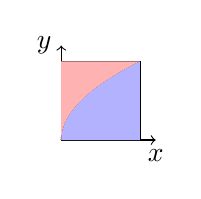
\begin{tikzpicture}
        % 绘制坐标轴
        \draw[->] (0,0) -- (1.2,0) node[below]{$x$};
        \draw[->] (0,0) -- (0,1.2) node[left]{$y$};

        % 绘制曲线 y = sqrt(x)
        \draw[domain=0:1,samples=100] plot (\x,{sqrt(\x)});

        % 绘制正方形 (0,0) 到 (1,1)
        \draw (0,0) rectangle (1,1);

        % 填充 D_2(蓝色)
        \fill[blue!30] (0,0) -- plot[domain=0:1,samples=100] (\x,{sqrt(\x)}) -- (1,0) -- cycle;

        % 填充剩余部分(红色)
        \fill[red!30] (0,1) -- plot[domain=0:1,samples=100] (\x,{sqrt(\x)}) -- (1,1) -- cycle;
        \end{tikzpicture}
    \end{center}
    显然蓝色区域$D_2$等于$D_1-D_{2'}$其中$D_{2'}$为红色区域即
    $$
    J_2=\iint_{D_1} - \iint_{D_{2'}}\sqrt{x-y}\d x\d y 
    $$
    不难发现在红色区域$y>x$是显然的,故$J_2>0$,同理可以得出$J_3<0$ 
    $$
    \fbox{$J_3<J_1<J_2$}
    $$
    \end{solution}
\end{enumerate}

\section{交换积分次序}

\begin{enumerate}[label=\arabic*.,start=3]
    \item (2001,数一)交换二次积分的积分次序:
    $\displaystyle\int_{-1}^0 dy\int_2^{1-y} f(x,y)dx$=\_\_\_\_
    
    \begin{solution}
    交换积分次序的题目,注意原函数的积分上下限即可,画图即可. 
    \begin{align*}
        \text{原式} &={\color{red} -}\int_{-1}^{0}\d y\int_{1-y}^{2}f(x,y)\d x \\
        &= -\int_{1}^{2}\d x\int_{1-x}^{0}f(x,y)\d y
    \end{align*}
    \end{solution}
    \newpage
    \item 二次积分$\displaystyle\int_{0}^{1}\d y\int_{y}^{1}\left(\frac{e^{x^2}}{x}-e^{y^2}\right)\d x$=\_\_\_\_
    \begin{solution}
    \begin{align*}
        \text{原式} &=\int_{0}^{1}\d y\int_{y}^{1}\frac{e^{x^2}}{x}\d x - \int_{0}^{1}\d y\int_{y}^{1}e^{y^2}\d y \\
        &=\int_{0}^{1}e^{x^2}\d x - \int_{0}^{1}(1-y)e^{y^2}\d y \\
        &=\int_{0}^{1}xe^{x^2}\d x\\
        &=\frac{1}{2}(e-1)
    \end{align*}
    \end{solution}
    
    \item 交换$\displaystyle I=\int_{-\frac{\pi}{4}}^{\frac{\pi}{2}}d\theta\int_0^{a\cos\theta}f(r,\theta)dr$的积分次序。
    
    \begin{solution}
    极坐标的积分换序,不要按照极坐标做就当成$x-y$做
    $$
    \text{原式} = \int_{0}^{\frac{\sqrt{2}}{2}a}\d r\int_{-\frac{\pi}{4}}^{\arccos{\frac{r}{a}}}f(r,\theta)\d \theta + 
    \int_{\frac{\sqrt{2}}{2}a}^{a}\d r\int_{-\arccos{\frac{r}{a}}}^{\arccos{\frac{r}{a}}}f(r,\theta)\d \theta
    $$
    \end{solution}

    \begin{tcolorbox}[title=什么时候要变化积分次序]
    第一种 - 出现典型的可积不可求的函数如
    $$
    \begin{cases}
        e^{\pm x^2},e^{\frac{1}{x}},\frac{1}{\ln{x}} \\
        \sin{x^2}, \sin{\frac{1}{x}},\fbox{$\frac{\sin{x}}{x}$} \\
        \cos{x^2}, \cos{\frac{1}{x}}, \fbox{$\frac{\cos{x}}{x}$} \\
    \end{cases}
    $$
    第二种 - 题目明确要求了要进行积分变换 \\
    第三种 - 积分区域和积分顺序显然不符合 \\
    第四种 - 题目给的积分正常做会非常难算 
    \end{tcolorbox}
\end{enumerate}

\section{二重积分的计算}
\begin{remark}
    $$
    \text{二重积分的计算}
    \begin{cases}
        \text{直角坐标系}\begin{cases}
            x\text{型}\\
            y\text{型}
        \end{cases} \\
        \text{极坐标}\qquad r\d r \\
        \text{性质}\begin{cases}
            \text{奇偶性} \\
            \text{轮换对称性} \\
        \end{cases} \\
        \text{形心公式} \iint_{D}x\d \sigma = \bar{x}S_D,\iint_{D}y\d \sigma = \bar{y}S_D \\
        \text{平移变换} \\
        {\color{red} \text{换元法-雅可比行列式}}
    \end{cases}
    $$
\end{remark}
\begin{enumerate}[label=\arabic*.,start=6]
    \item (2011,数一、数二)已知函数$f(x,y)$具有二阶连续偏导数,且$f(1,y)=0$,$f(x,1)=0$,$\iint_D f(x,y)dxdy=a$,其中$D=\{(x,y)|0\leq x\leq 1,0\leq y\leq 1\}$,计算二重积分
    \begin{align*}
        I=\iint_D xyf_{xy}''(x,y)\d x\d y.
    \end{align*}
    
    \begin{solution}
    有题设可知$f'_x(x,1)=f'_y(1,y)=0$ 
    \begin{align*}
        \text{原式} &= \int_{0}^{1}\d x\int_{0}^{1}xyf''_{xy}(x,y)\d y \\
        &=\int_{0}^{1}x\d x\int_{0}^{1}y\d f'_x(x,y) \\
        &=-\int_{0}^{1}x\d x\int_{0}^{1}f'_x(x,y)\d y \\
        &=-\int_{0}^{1}\d y\int_{0}^{1}xf'(x,y)\d x \\
        &=\iint_{D}f(x,y)\d x\d y = a
    \end{align*}
    \end{solution}
    
    \item 计算$\iint_D\sqrt{|y-x^2|}dxdy$,其中$D=\{(x,y)|-1\leq x\leq 1,0\leq y\leq 2\}$。
    
    \begin{solution}
    积分区域如下所示
    \begin{center}
        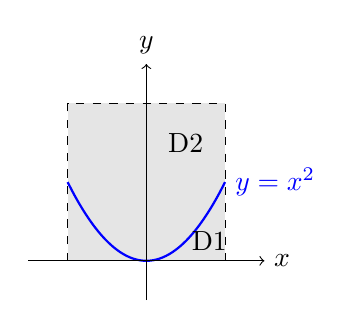
\begin{tikzpicture}[scale=1]
            % 坐标轴
            \fill[gray!20] (-1,0) rectangle (1,2);
            \draw[dashed] (-1,0) -- (-1,2) -- (1,2) -- (1,0);
            \draw[blue, thick, domain=-1:1, smooth] plot (\x, {\x*\x}) node[right]{$y = x^2$};
            \draw[->] (-1.5,0) -- (1.5,0) node[right]{$x$};
            \draw[->] (0,-0.5) -- (0,2.5) node[above]{$y$};
            \node at (0.8, 0.25) {D1};
            \node at (0.5, 1.5) {D2};
        \end{tikzpicture}
    \end{center}
    显然图像关于$x$对称,且原函数关于$y$是偶数故由对称性可知
    \begin{align*}
        \text{原式} &= 2\iint_{D_1}\sqrt{x^2-y}\d x\d y + 2\iint_{D2}\sqrt{y-x^2}\d x\d y \\
        &=2\int_{0}^{1}\d x\int_{0}^{x^2}\sqrt{x^2 - y}\d y + 2\int_{0}^{1}\d x\int_{x^2}^{2}\sqrt{y-x^2}\d y \\
        2\int_{0}^{1}\d x\int_{0}^{x^2}\sqrt{x^2 - y}\d y &=\frac{4}{3}\int_{0}^{1}x^3\d x =\frac{1}{3} \\
        2\int_{0}^{1}\d x\int_{x^2}^{2}\sqrt{y-x^2}\d y &= \frac{4}{3}\int_{0}^{1}(2-x^2)^{\frac{3}{2}}\d x \\
        &\xlongequal{x=\sqrt{2}\sin{t}}\frac{16}{3}\int_{0}^{\frac{\pi}{4}}\cos^4{t}\d t \\
        &=\frac{16}{3}\int_{0}^{\frac{\pi}{4}}(\frac{1+\cos{2t}}{2})^2\d t \\
        &=\frac{2}{3}\int_{0}^{\frac{\pi}{2}}(1+\cos{t})^2\d t \\
        &= \frac{\pi}{2}+\frac{4}{3} \\
        \text{原式} &= \fbox{$\displaystyle\frac{5}{3} + \frac{\pi}{2}$}
    \end{align*}
    \end{solution}
    
    \item (2018,数二)设平面区域$D$由曲线$\begin{cases}x=t-\sin t \\ y=1-\cos t\end{cases}(0\leq t\leq 2\pi)$与$x$轴围成,计算二重积分$\iint_D(x+2y)dxdy$。
    
    \begin{solution}
    题设参数方程即\underline{摆线}图像如图所示,关键性质为其关于$x=\pi$对称
    \begin{center}
        \begin{tikzpicture}[scale=1]
        \draw[->] (-0.5,0) -- (7,0) node[right]{$x$};
        \draw[->] (0,-0.5) -- (0,2.5) node[above]{$y$};
        \draw[domain=0:2*pi, samples=100, smooth, thick, blue] 
            plot ({\x - sin(\x r)}, {1 - cos(\x r)});
        \filldraw (0,0) circle (1pt) node[below left]{$(0,0)$};
        \filldraw ({2*pi - sin(2*pi r)}, {1 - cos(2*pi r)}) circle (1pt) node[above right]{$(2\pi,1)$};
        \end{tikzpicture}
    \end{center}
    由于摆线关于$x=\pi$对称由形心公式有
    $$
    \iint_{D}x\d x\d y = \pi\iint_{D}\d x\d y
    $$
    故有
    \begin{align*}
        \text{原式} &= \iint_{D}(\pi+2y)\d x\d y \\
        &=\int_{0}^{2\pi}\d x\int_{0}^{y(x)}(\pi + 2y)\d y\\
        &=\int_{0}^{2\pi}\left[\pi y(x)+y^2(x)\right]\d x \\
        &\xlongequal{x=t-\sin{t}} \int_{0}^{2\pi}\left[\pi(1-\cos{t})+(1-\cos{t})^2\right](1-\cos{t})\d t \\
        &=3\pi^2+5\pi
    \end{align*}
    \end{solution}
    
    \item (2007,数二、数三)设二元函数
    \begin{align*}
        f(x,y)=\begin{cases}
            x^2, & |x|+|y|\leq 1 \\
            \frac{1}{\sqrt{x^2+y^2}}, & 1<|x|+|y|\leq 2
        \end{cases}
    \end{align*}
    计算二重积分$\iint_D f(x,y)dxdy$,其中$D=\{(x,y)||x|+|y|\leq 2\}$。
    
    \begin{solution}
        积分区域如图所示
    \begin{center}
        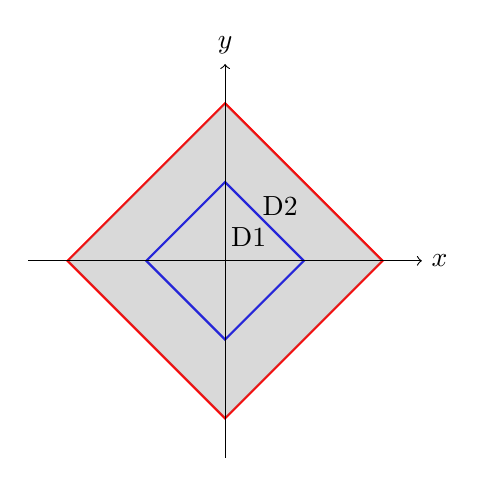
\begin{tikzpicture}[scale=1]
        \draw[thick, blue] (1,0) -- (0,1) -- (-1,0) -- (0,-1) -- cycle;
        \draw[thick, red] (2,0) -- (0,2) -- (-2,0) -- (0,-2) -- cycle;
        \fill[gray, opacity=0.3] 
            (2,0) -- (0,2) -- (-2,0) -- (0,-2) -- cycle 
            -- (1,0) -- (0,1) -- (-1,0) -- (0,-1) -- cycle -- cycle;
        \draw[->] (-2.5,0) -- (2.5,0) node[right] {$x$};
        \draw[->] (0,-2.5) -- (0,2.5) node[above] {$y$};
        \node at (0.3, 0.3) {D1};
        \node at (0.7,0.7) {D2};
        \end{tikzpicture}
    \end{center}
    由奇偶性可知
    $$
    \text{原式} =4(\iint_{D_1}x^2\d x\d y + \iint_{D_2}\frac{1}{\sqrt{x^2+y^2}}\d x\d y)
    $$
    其中
    $$
    \iint_{D_1}x^2\d x\d y = \int_{0}^{1}\d x\int_{0}^{1-x}x^2\d x\d y = \frac{1}{12}
    $$
    \begin{align*}
        \iint_{D_2}\frac{1}{\sqrt{x^2+y^2}}\d x\d y &=\int_{0}^{\frac{\pi}{2}}\d \theta\int_{\frac{1}{\sin{\theta}+\cos{\theta}}}^{\frac{2}{\sin{\theta}+\cos{\theta}}}
        \frac{1}{r}r\cdot\d r \\
        &=\int_{0}^{\frac{\pi}{2}}\frac{\d \theta}{\sin\theta+\cos\theta} \\
        \text{方法一}\ \text{万能代换} & = \sqrt{2}\ln{(\sqrt{2}+1)} \\
        \text{方法二}\ \text{三角公式} &= \int_{0}^{\frac{\pi}{2}}\frac{\d \theta}{\color{red}\sqrt{2}\sin{(\theta+\frac{\pi}{4})}} \\
        &=\frac{1}{\sqrt{2}}\ln{\left|\csc{(\theta+\frac{\pi}{4})}-\cot{(\theta+\frac{\pi}{4})}\right|}\bigg|^{\frac{\pi}{2}}_{0} \\
        &=\sqrt{2}\ln{(\sqrt{2}+1)}
    \end{align*}
    综上
    $$
    \text{原式} = 4(\frac{1}{12}+\sqrt{2}\ln{(\sqrt{2}+1)})
    $$
    \end{solution}
    
    \item (2014,数二、数三)设平面区域$D=\{(x,y)|1\leq x^2+y^2\leq 4,x\geq 0,y\geq 0\}$,计算
    \begin{align*}
        \iint_D\frac{x\sin(\pi\sqrt{x^2+y^2})}{x+y}\d x\d y.
    \end{align*}
    
    \begin{solution}
    积分区域如下所示
    \begin{center}
        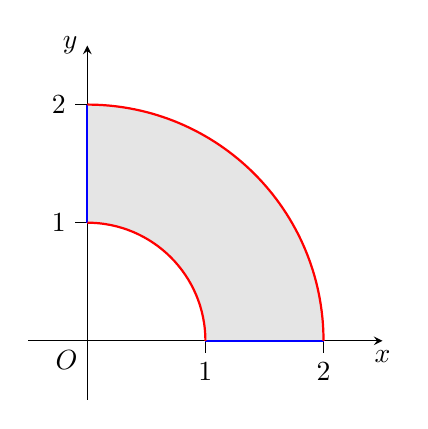
\begin{tikzpicture}[scale=1.5, >=stealth]
        \draw[->] (-0.5,0) -- (2.5,0) node[below] {$x$};
        \draw[->] (0,-0.5) -- (0,2.5) node[left] {$y$};
        \node[below left] at (0,0) {$O$};
        \foreach \x in {1,2} {
            \draw (\x,0) -- (\x,-0.1) node[below] {$\x$};
        }
        \foreach \y in {1,2} {
            \draw (0,\y) -- (-0.1,\y) node[left] {$\y$};
        }
        \fill[gray!20] 
            (2,0) arc (0:90:2)   % 外圆弧 (半径2, 从x轴到y轴)
            -- (0,1)             % 沿y轴从(0,2)移动到(0,1)
            arc (90:0:1)         % 内圆弧 (半径1, 从y轴到x轴)
            -- cycle;            % 沿x轴从(1,0)回到(2,0)
        \draw[thick, blue] (1,0) -- (2,0);  % x轴边界
        \draw[thick, blue] (0,1) -- (0,2);  % y轴边界
        \draw[thick, red] (1,0) arc (0:90:1);  % 内圆边界 (半径1)
        \draw[thick, red] (2,0) arc (0:90:2);  % 外圆边界 (半径2)
    \end{tikzpicture}
    \end{center}
    (方法一) 转换为极坐标,此时积分为
    \begin{align*}
        \text{原式} &=\int_{0}^{\frac{\pi}{2}}\d \theta\int_{1}^{2}\frac{r\cos{\theta}\sin{(\pi r)}}{r(\sin\theta+\cos\theta)}r\cdot\d r \\
        &=\int_{0}^{\frac{\pi}{2}}\frac{\cos\theta}{\sin\theta+\cos\theta}\d\theta\int_{1}^{2}r\sin(\pi r)\d r \\
        &=\frac{\pi}{4}\cdot\frac{-3}{\pi} = -\frac{3}{4}
    \end{align*}
    (方法二) 考虑轮换对称性,此时积分为
    \begin{align*}
        I &=\frac{1}{2}\iint_{D}\sin{(\pi\sqrt{x^2+y^2})}\d x\d y\\
        &=\frac{1}{2}\int_{0}^{\frac{\pi}{2}}\d \theta\int_{1}^{2}\sin{(\pi r)}r\cdot\d r \\
        &=\frac{\pi}{4}\cdot(-\frac{3}{\pi}) = -\frac{3}{4}
    \end{align*}
    \end{solution}
    
    \item (2019,数二)已知平面区域$D=\{(x,y)||x|\leq y,(x^2+y^2)^3\leq y^4\}$,计算二重积分
    \begin{align*}
        \iint_D\frac{x+y}{\sqrt{x^2+y^2}}\d x\d y.
    \end{align*}
    
    \begin{solution}
    \newpage
    \end{solution}
\end{enumerate}

\section{其他题型}

\begin{enumerate}[label=\arabic*.,start=12]
    \item (2010,数二)计算二重积分$\displaystyle I=\iint_D r^2\sin\theta\sqrt{1-r^2\cos 2\theta} drd\theta$ \\
    其中$\displaystyle D=\left\{(r,\theta)\mid 0\leq r\leq\sec{\theta},0\leq\theta\leq\frac{\pi}{4}\right\}$
    
    \begin{solution}
    \newpage
    \end{solution}
    
    \item (2009,数二、数三)计算二重积分$\iint_D(x-y)dxdy$\\
    其中$\displaystyle D=\{(x,y)|(x-1)^2+(y-1)^2\leq 2,y\geq x\}$.
    
    \begin{solution}
    \newpage
    \end{solution}
\end{enumerate}

\ifx\allfiles\undefined
\end{document}
\fi